\documentclass[letterpaper,12pt]{book}

% \pdfpagewidth 8.5in
% \pdfpageheight 11in

\usepackage[english]{babel}
\usepackage[english]{minitoc}
\usepackage[OT1]{fontenc}
\usepackage[isolatin]{inputenc}
\usepackage{mltex}
\usepackage{longtable}
\usepackage{makeidx}
\usepackage{url}
%\usepackage{MnSymbol}
%\usepackage{draftcopy}
%\usepackage{lastpage}
\addtolength{\topmargin}{-0.5in}
\addtolength{\oddsidemargin}{-2in}
\addtolength{\textwidth}{1in}
\addtolength{\textheight}{2in}
%
%\ifdefined\DEBUG
%    DEBUG was on
%\else
%   DEBUG was off
%\fi
% Voir pour les figures PS v.s. PDF
%\ifdefined\FIGURE
%    DEBUG was on
%\else
%   DEBUG was off
%\fi
% pdflatex "\def\FIGURE{}\input{la_figure.png}'' file.tex
%
%\ifdefined\KINDLE
%\usepackage[paperwidth=13cm, paperheight=18cm, top=1cm, left=0.2cm, right=0.2cm, bottom=1.5cm, includefoot]{geometry}
%\fi
%\ifx\KINDLE\undefined
%\usepackage[paperwidth=13cm, paperheight=18cm, top=1cm, left=0.2cm, right=0.2cm, bottom=1.5cm, includefoot]{geometry}
%\else
%\fi
%
% curriculum vitae
%
\newcommand{\resitem}[1]{\item #1 \vspace{-2pt}}
\newcommand{\resheading}[1]{{\large \parashade[.9]{sharpcorners}{\textbf{#1 \vphantom{p\^{E}}}}}}
\newcommand{\ressubheading}[4]{
  \vspace{+7pt}
  \begin{tabular*}{6.5in}{l@{\extracolsep{\fill}}r}
    \textbf{#1} & #2 \\
    \textit{#3} & \textit{#4} \\
  \end{tabular*}
  \vspace{-3pt}}
%
% informations AQ
%
\newcommand{\titre}{Validation/qualification pour  le code Monte-Carlo
  Tripoli4~: r\'esultats} 
\newcommand{\auteur}{\mbox{Yann Cobigo}}
\newcommand{\Page}{\thepage/\pageref{LastPage}}
\newcommand{\Date}{\today}
\newcommand{\numserma}{00-0000}
\newcommand{\indicerapport}{A}
\newcommand{\LABORATOIRE}{LTSD}
\newcommand{\Tripoli}{$\times$}
\newcommand{\Darwin}{$\times$}
\newcommand{\Narmer}{}
\newcommand{\Minutes}{}
\newcommand{\Releve}{$\times$}
%
% titre  LaTeX :  si on deicommante  les trois lignes  suivantes, il
%  faut  decommanter la ligne maketitle qq lignes suivantes.
%
\newcommand{\Nom}{\titre}
\newcommand{\AUTEUR}{\auteur}
\newcommand{\PAGE}{\Page}
\newcommand{\DATE}{\Date}
\newcommand{\NUMRAPPORT}{\numserma}
\newcommand{\INDICERAPPORT}{\indicerapport}
\newcommand{\SERVICE}{SERMA}
\newcommand{\TRIPOLI}{\Tripoli}
\newcommand{\DARWIN}{\Darwin}
\newcommand{\NARMER}{\Narmer}
\newcommand{\MINUTES}{\Minutes}
%
% MACROS MATHEMATIQUES
%
\newcommand{\FIJEE}{{\it Forward-Inverse~/ Electro-Encephalogram}}
\newcommand{\FEM}{finite element method}
\newcommand{\PED}{partial differential equations}
% Brain
\newcommand{\GM}{gray-matter}
\newcommand{\WM}{white-matter}
\newcommand{\CSF}{cerebrospinal fluid}
% Software
\newcommand{\CGAL}{Computational Geometry Algorithms Library (CGAL)}
\newcommand{\VTK}{Visualization Toolkit (VTK)}
\newcommand{\FENICS}{FEniCS Project}
\newcommand{\FREESURFER}{FreeSurfer}
% format
\newcommand{\INRIMAGE}{INR Image (INRIMAGE)}
\newcommand{\STL}{stereolithography (STL)}
\newcommand{\NIFTI}{Neuroimaging Informatics Technology Initiative (NIFTI)}
%
\def\ci{\perp\!\!\!\perp} % Conditional independence
%
\usepackage{longtable}
\usepackage{graphics}
%\usepackage{/usr/share/texmf/tex/latex/fancyheadings/fancyheadings}
\usepackage{/usr/share/texmf/tex/latex/fancyhdr/fancyhdr}
\usepackage{OtherRapport/en-tete}
\usepackage{lastpage}
%
% In amsmath and esint some mathematics function are declared in both packages
% We have to save them in the first package...
%
\usepackage{savesym}
\usepackage{amsmath}
\savesymbol{iint}
\usepackage{amssymb}
\usepackage{esint}
\usepackage{graphicx}
\pagestyle{fancy}
% index information
\makeindex
%
\begin{document}
%\maketitle
\begin{quote}
%
\begin{picture}(19.1,3.5)(0,0)
         \put(0.14,3.0){\framebox(8.0,0.5){}}
         \put(0.5,3.1){\bf \large Client~: Gazzaley Laboratory}
         \put(0.14,1.99){\framebox(8.0,1.0){}}
         \put(0.5,2.55){\bf \large Demande: scientific software}
         \put(0.5,2.09){\bf \large Location: UC San Francisco}
         \put(9,3.0) {\framebox(8.6,0.5){\bf Reference: GazzLab/TECH/001/A}}
         \put(9,2.52) {\framebox(0.3,0.3){}}
         \put(9.,2.57){\Minutes}
         \put(9.5,2.52){\bf Meeting repport}
         \put(9,2.06) {\framebox(0.3,0.3){}}
         \put(9.,2.11){\Releve}
         \put(9.5,2.06){\bf Project repport}
\end{picture}

\vspace*{2cm}

\begin{center}
\textsc{\textbf{\LARGE Fijee:~\FIJEE{} software}}
\end{center}

\vspace*{2cm}

Editor:\\\hspace*{4cm}
\begin{tabular}{l}
Dr. Morgan Hough\\
\end{tabular}
\vspace*{1cm}

Writer:\\\hspace*{4cm}
\begin{tabular}{l}
Yann Cobigo\\
\end{tabular}

\vspace*{2cm}
\begin{center}
\textsc{\textbf{\large Version history}}
\end{center}

\vspace*{1cm}
\begin{center}
  \begin{tabular}{|c|c|c|c|} \hline
    Date & Indice & Writer version & Modifications asked \\ \hline
    12/11/2008 & A & Y. Cobigo & Cr�ation de la premi�re version \\ \hline
  \end{tabular}
\end{center}
%
\newpage
%
\small
\vspace*{3cm}
\dominitoc
\tableofcontents
%
\newpage
%
\frontmatter
\chapter{Introduction}
\minitoc

\cite{ANS-EELWFM}


%
%
%
\mainmatter
%
\part{Forward method principes}
\chapter{Dipole modelisation in the brain}
\minitoc
%\include{chapters/Probabilite}
%
\chapter{Tetrahedrization mesh of a subject}
\minitoc
A mesh is a representation of an object (a volume or shape in the plane) by a finite number of simple elements. Among meshes, simplicial meshes\index{simplicial meshes} are built from simplices. A simplicial mesh is a collection of simplices, with disjoint interiors, such as the intersection of two simplices is either empty or a simplex with lower dimension. \\
The simplicial meshes are very popular for representing surfaces, volumes. They are suitable for numerical simulation. For instance, the finite element method allows the approximate solution of systems of partial differential equations ({\it c.f.} section~\ref{FEM}) using meshes. \\
The generation of realistic geometric patient models from high-resolution medical images is of great significance in many clinical and research applications. 

\newpage

%-------------------------------------------------------------------------------

\section{Mathematical background}

Voronoi diagrams are structures encoding the proximity relationships between objects. Delaunay triangulations, which are geometrically dual to Voronoi diagrams, are a classical tool of computational geometry\index{computational geometry}, in the field of mesh generation\index{mesh generation} and mesh processing due to its optimality properties.\\
We now turn to the following problem: $E$ is a set of points in the plane or space, {\it what is the best triangulation of E?} The answer this question three properties of the triangulation are particularly sought: \\

\begin {itemize}
\item the algorithm must be robust (adding or deleting a point of $E$ does not require a complete change in the triangulation);
\item the algorithm must be fast to compute;
\item the algorithm must contain a minimum of elongated triangles (slivers). \\
\end {itemize}

A sliver is a tetrahedron whose four vertices lie close to a plane and whose projection to that plane is a quadrilateral with no short edge. Such tetrahedra have a good radiusedge ratio but a very poor radius-radius ratio (ratio between circumradius and radius of largest contained sphere). Unfortunately, the latter measure typically influences the numerical conditioning of finite element methods. In order to remove slivers from our volume meshes, we use a post processing step called sliver exudation [21]. This algorithm is efficient in practice and generates almost sliver-free meshes.

%I will restrict the case of discrete surfaces, that is to say, defined from a finite number of points.

\subsection{Topological space}

Topological aproximation: it is necessary to determine a mesh topology similar to the target object. The edge of a solid object must be a subset of triangles of the mesh, homeomorphic\footnote{A homeomorphism, or topological isomorphism or bicontinuous function, is a continuous function between topological spaces that has a continuous inverse function.} itself at the edge of the object. In addition, if the object has internal partitions to separate out different areas, the mesh must represent these partitions.\\

In this section we summarize some mathematical definitions of mesh generation.

\paragraph{Definition - Topological space}\index{topological space}
{
\it A topological space is a set $\mathbb{X}$ and a system $X$ of subsets of $\mathbb{X}$ such that:
\begin{itemize}
\item  $\varnothing$, $X \in \mathbb{X}$;
\item  a union of elements of $X$ is in $\mathbb{X}$ ;
\item  a finite intersection of elements in $X$ is in $\mathbb{X}$.
\end{itemize}

$X$ is called a topology and elements of $X$ are called open set in $\mathbb{X}$. %A topological subspace ($Y$, $\mathbb{Y}$) of ($X$, $\mathbb {X}$) consists of a subset of $\mathbb{Y} \subset \mathbb{X}$ and the topology of the subspace defined by $Y = \{\mathbb{Y} \cap A, A \in X \}$
}

\paragraph{Definition - Simplex}\index{simplex}
{
\it Let $\{e_{0},~e_{1}, \dots,~ e_{n} \}$ be a set of $n+1$ linearly independent points in a Euclidean space\footnote{the concept of an Euclidean space encompasses Euclidean plane and the three-dimensional space of Euclidean geometry as spaces of dimensions 2 and 3 respectively.}\index{Euclidean space} $\mathbb{E}^{m}$ where $m \ge n \ge 0$. We call a $n$-simplex, with vertices $e_{0},~e_ {1},~\dots, e_{n}$, the hull $\sigma $ of these convex points. $n$ is the dimension of $\sigma$. The set $-1$-simplex is the empty set.
}

\paragraph{Example}
{
In $\mathbb{R}^{3}$, a $0$-simplex is a vertex, a $1$-simplex is an edge, a $2$-simplex is a triangle and a $3$-simplex is a tetrahedron.
}

\paragraph{Definition - Face}\index{face}
{
\it Let $S$ be a set of linearly independent points and $\sigma$ its convex hull. Then the convex hull $\tau$ of any subset $T$ of $S$ is a simplex subset of $\sigma$. We say that $\tau$ is a face of $\sigma$, and we write $\tau \le \sigma$.
}

\paragraph{Definition - Simplicial complex}\index{simplicial complex}
{
\it A simplicial complex $K$ is a collection of faces of a finite number of simplices, such as: if $\sigma$ is in $K$ then any face of $\sigma$ is in $K$, and if $\sigma$ and $\nu$ are in $K$ then theire intersection is a face of both $\sigma$ and $\nu$. The dimension of a simplicial complex is the size of the largest simplex.
}

In other words, a simplicial complex is a geometric object describing some topological spaces by generalizing the concept of triangulation of a surface. Such an object is presented as a graph with vertices connected by edges, which can be attached on the triangular faces.

\paragraph{Definition - Polyhedron}\index{polyhedron}
{
\it Let $K$ be a simplicial complex in $\mathbb{R}^{n}$. The union $|K|$ of all simplices of $K$ with the topology of subspace of $\mathbb{R}^{n}$ is called the polyhedron $K$.
}

\paragraph{Definition - Triangulation}\index{Triangulation}
{
\it The triangulation of a topological space $X$ is a simplicial complex $K$ whose polyhedron $|K|$ is homeomorphic to $X$. If a simplicial complex exists, we say that $X$ is triangulated.
}

\subsection{Voronoi Diagram}

The Voronoi diagram\index{Voronoi diagram}, also called {\it Dirichlet tessellation}\index{Dirichlet tessellation}, with the convex hull are a practical geometric structures. It was introduced in  $\mathbb {R}^{2}$ and $\mathbb{R}^{3}$ by the German mathematician Johann Peter Gustav Lejeune Dirichlet (1805-1859) in 1850. The Russian-Ukrainian mathematician Georgy Voronoi (1868-1908) formalized this notion in the general case in 1908.\\

Let $E$ be a Euclidean vector space and $P = \{p_{i}, 1 \le i \le n\} $ be a finite set of points of $E$.

\paragraph{Definition - Voronoi cell}
{
\it A Voronoi cell of the point $p_{i} \in P$, denoted $C_{i}$, is the set of points of $E$ the closest to $p_ {i}$ than any other point of $P$:
$$
C_{i} = \{q \in E,~\forall j \ne i~~/~~ \| qp_{i} \| \le \| qp_{j} \| \}
$$

The point $p_{i}$ associated to the cell $C_{i}$ is called the site of the cell.
}       

\paragraph{Definition - Voronoi Diagram}
{
\it A Voronoi diagram of the $P$, denoted $Vor (P)$, is the subdivision of $E$ in $C_{i}$ cells associated with points $p_{i}$ of $P$:

$
Vor (P) = \bigcup_{p_{i} \in P} C_{i}
$
}

\paragraph{Definition - vertex, edge and face of Voronoi}
{
\it Let $d$ be the dimension of $E$. The intersection of $d + 1$ Voronoi cells, if not empty, is called a Voronoi vertex. The intersection of $d$ Voronoi cells, if not empty, is called Voronoi edge. The intersection $i$ Voronoi cells, $ 2 \le i \le d - 1$, if it is not empty, is called Voronoi face.
}

\paragraph{Properties}
{
\begin {itemize}
\item A Voronoi edge separating two cells $C_{i}$ and $C_{j}$ is given by the bisection of the segment $p_{i}p_{j}$.
\item The Voronoi vertex separating three cells $C_{i}$, $C_{j}$ and $C_{k}$ is the center of the circle circumscribing the triangle with vertices $p_{i}$, $p_{j}$ and $p_{k}$.
\item A Voronoi cell, if it is bounded, is a convex polygon.
\end {itemize}
}


\subsection{Delaunay Triangulation}

Delaunay meshing is recognized as one of the most powerful techniques for generating surface and volume meshes with guaranteed quality. The notion of Delaunay triangulation was proposed in 1934 by a student of Russian mathematician Georgy Voronoi: Boris Delaunay. \\
The Delaunay triangulation of a space $E$ is defined as the geometric dual of the Voronoi diagram: there is an edge between two points $p_{i}$ and $p_{j}$ in the Delaunay triangulation if and only if their Voronoi cells $V(p_{i})$ and $V(p_{j})$ have a non-empty intersection. It yields a triangulation of the space $E$, that is to say a partition of the convex hull of $E$ into $d$-dimensional simplices (i.e. into triangles in 2D, into tetrahedra in 3D and so on). The fundamental property of the Delaunay triangulation is called the empty circle (empty sphere in 3D) property: in 2D (resp. in 3D), a triangle (resp. tetrahedron) belongs to the Delaunay triangulation if and only if its circumcircle (resp. circumsphere) does not contain any other points of $E$ in its interior. \\

\paragraph{Definition - Delaunay Triangulation}
{
\it A Delaunay triangulation of the set $P$, denoted $Del(P)$, is the dual of the Voronoi diagram of $P$: vertices of the Delaunay triangulation are the points $p_{i} \in P$, and two vertices are connected by an edge in triangulation if the corresponding Voronoi cells are adjacent.
}

\paragraph{Note:}
{
Although this definition is valid in the case of a Euclidean space $E$ of any dimension, the term triangulation refers to the case plan. In the case of $\mathbb{R}^{3}$, sometimes called Delaunay tetrahedralization.
}

\paragraph{Definition - Vertex, edge of Delaunay}
{
\it The vertices of a Delaunay triangulation are called vertices of Delaunay. If $E = \mathbb{R}^{2}$, the edges of a Delaunay triangulation is called Delaunay edges.
}

\paragraph{Properties}
{
The cercle centered on a Voronoi site and passing through the three neighboring sites $p_{i}$, $p_{j}$ and $p_{k}$ is the circumcircle of the Delaunay triangle $p_{i}p_{j}p_{k}$.
}


\paragraph{Theorem - Characterization of Delaunay triangulations}
{
\it Let $p_{i}$, $p_{j}$ and $p_{k}$ three points $P$. Then the triangle with vertices $p_{i}$, $p_{j}$ and $p_{k}$ is a triangle of the Delaunay triangulation of $P$ if and only if the circumcircle of a triangle that contains no another point of $P$.
}

\paragraph{Properties}
{
Let $p_{i}$ and $p_{j}$ two points $P$. Then $p_{i}p_{j}$ segment is an edge of the Delaunay triangulation of $P$ if and only if there is a circle passing through $p_{i}$ and $p_{j}$ such that the corresponding disc contains no other point $P$.
}

\subsection{Restricted Delaunay triangulation}

\newpage{}

%-------------------------------------------------------------------------------

\section{\FIJEE{}'s mesh}

However, due to the lack of reliable fully-automated tools for the unstructured discretization of medical datasets, simplistic geometric models are still of wide use. \\
The simplicial meshes are good tools for the finite element method, and more generally for many computational methods for modeling physical systems. However, the creation of such meshes is sometimes problematic. Indeed, the generation of a mesh representing a continuous and appropriate form for numerical simulation or visualization, can be demanding for time and memory resources. In complicated cases, it may be impossible to generate a mesh without manual intervention to meet the needs of the calculation.\\
Similarly, in the EEG/MEG source localization problem using the boundary element method (BEM), as pointed out in [2], popular simplistic head models consisting of nested tissue layers may yield a significantly lower accuracy than realistic models featuring multiple junctions.\\


\FIJEE{} allows the electric potential mapping at the surface of the skull. This calculation is based on solving the Poisson equation with the \FEM{}. The production of the mesh used by the \FEM{} is achieved by \CGAL{}. Selecting \CGAL{} for this task was based on several criteria:


\begin{itemize}
\item {\bf licence}
\item sophisticated developpement in C++ language; flexible and easy to link to \FIJEE{};
\item efficient forum support;
\item large toolkit available;
\item mesh production on complexe geometry.
\end{itemize}

For the latter, \CGAL{} has two very important features used by \FIJEE{}. The first is the ability to create an implicit functions from a set of points and normals. The second is the mesh generation modularity (heterogeneous mesh size control) from the labeled volume image of the head.  It offers easy control over the size and shape of mesh tetrahedra.\\

\subsection{Implicite surface}

{\bf intro from CGAL, voir s'il y a un article}\\
{\bf Faire le même topo que freesurfer pour le logiciel produisant skull/scalp}\\

\FREESURFER{} is a software known for the studies of \WM{} and \GM{}. \FREESURFER{} provides a detailed \WM{} and \GM{} surface meshes. \texttt{mris\_convert}, tool from \FREESURFER{}'s toolkit, allows the conversion of these meshes in the form \STL{}. From \STL{} format via \CGAL{}, it become possible to build implicite functions in purpose to produice labeled  volumes. \\
Before selecting \CGAL{} to create implicit surafaces, tests were made with other algorithms. In particular, {\bf give the algorithm} used by \VTK{}. The results, {\bf show results} offer low efficiency and reliability. \\

\subsection{Labeled volumes image}

{\bf intro from CGAL, voir s'il y a un article}\\
\FIJEE{} offers the possibility to create a representation of labeled volumes of a patient's head, in a completely automatic way. This image, in three dimensions and \INRIMAGE{}\footnote{http://serdis.dis.ulpgc.es/~krissian/InrView1/IOformat.html} format, is produced using implicit surfaces for the sclap, skull, \CSF{}, \GM{} and \WM{}. The subcortical parts of the image are extracted frome \texttt{aseg.nii} (\NIFTI{} format) a \FREESURFER{}'s output. \\
The image \INRIMAGE{} is provided as input to the \CGAL{}'s {\it oracle} for the production of three-dimensional volume meshes conforming different anatomical parts of the head.

\paragraph{To review - High-Quality Consistent Meshing of Multi-Label Datasets}
{


require geometrically-accurate and topologically-correct models. 


While different strategies can be used to obtain realistic geometric models from labeled medical datasets, few of them offer sufficient flexibility: handling of data coming from different sources, control over the density and quality of the mesh elements. Also, most existing approaches have been designed to extract surface meshes corresponding to boundaries between labeled anatomical structures, hence necessitating post-processing steps to generate volume meshes needed by finite element methods.

 It offers easy control over the size and shape of mesh elements, for instance through a (possibly non-uniform) sizing field.

Our work builds on some recent provably correct Delaunay-based algorithms for meshing smooth surfaces [14] and volumes bounded by such surfaces [15]. These two algorithms are proven to terminate and to construct good-quality meshes, while offering bounds on the approximation accuracy of the original boundary and on the size of the output mesh. The refinement process is controlled by highly customizable quality criteria on triangular facets and on tetrahedra. A notable feature of the method of Boissonnat and Oudot [14] is that the surface needs only to be known through an {\it oracle}\footnote{The domain is input to the mesh generation function, as a domain class, often called the oracle, that provides predicates and constructors related to the domain, the subdomains, the boundary surface patches and also the 0 and 1-dimensional exposed features, if any. Mainly, the oracle provides a predicate to test if a given query point belongs to the domain or not and to find in which subdomain it lies in the affirmative case.} that, given a line segment, detects whether the segment intersects the surface and, in the affirmative, returns an intersection point. This makes the algorithm useful in a wide variety of contexts and for a large class of surfaces. Very recently, Oudot, Rineau and Yvinec [15] have proposed to combine the latter Delaunay-based surface mesher with a Delaunay refinement volume mesher [16].

Our work extends the method of Boissonnat and Oudot [14] and the method of Oudot, Rineau and Yvinec [15] to the case of multi-label partitions, so that they can be applied to the generation of high-quality geometric models from labeled medical datasets. To that end, we define a partition of Delaunay tetrahedra induced by a space subdivision. It is related to the concept of restricted Delaunay triangulation, borrowed from computational geometry. In our approach, the subdivision of the domain of interest is approximated by a discrete partition of the Delaunay tetrahedralization of a point set: each Delaunay tetrahedron is labeled with one adequate tissue type. Output surface meshes are composed of the triangular facets adjacent to two tetrahedra having different labels. The point set is iteratively refined until it forms a good sample of the boundaries between the different anatomical structures, and, if a quality volume mesh is desired, a good sample of their interior.

Another notable feature of our approach is that the continuous partition need not to be represented explicitly. It is known only through a {\it labeling oracle} that, given a point in space, answers which tissue it belongs to. This makes our approach applicable to virtually any combination of data sources, including labeled 3D images, polyhedral surfaces, unstructured volume meshes, fuzzy membership functions, possibly having different resolutions and different coordinate systems. The different data sources may even be inconsistent with each other due to noise or discretization artefacts. In this case, the {\it labeling oracle} has the responsibility of resolving the conflicts using some user defined rules. As a result, our meshing algorithm is not affected by the heterogeneity and possible inconsistency of the input datasets. Finally, another major advantage of our approach is that the customizable quality criteria on boundary facets and/or on tetrahedra can be tuned independently for the different anatomical structures.


Experiment 2: Non-uniform surface meshing. In the three following experiments, we use some segmented brain data which were automatically generated from a T1-weighted magnetic resonance (MR) image using FreeSurfer's Whole Brain Segmentation tool [25]. The second experiment demonstrates the ability of our algorithm to produce surface meshes with non-uniform resolution (Fig. 3-Right). The facet size criterion was chosen to be spatially-varying so that the occipital cortex would be more finely sampled than the frontal cortex. Although for clarity, only four surfaces are displayed (for each hemisphere, the cortical and cerebellum surfaces), a total number of 72 tissues were meshed using the aforementioned criteria.

}

\newpage

%-------------------------------------------------------------------------------

\section{To review}

\paragraph{Meshing Volumes Bounded by Piecewise Smooth Surfaces~\cite{LRineau2007}}{

La meilleure façon d'améliorer ce compromis est de créer un maillage avec des tailles d'éléments localement adaptés à la précision nécessaire. La forme des éléments d'un maillage simplicial est capitale, pour les applications de calcul. Dans les méthodes de résolution approchée d'équations différentielles, à la fois les grands angles et les petits angles doivent être évités [She02b, She]. L'erreur d'approximation de la solution dépend principalement de la taille des éléments. Cependant, pour une taille d'éléments donnée, la présence de grands angles dans le maillage augmente l'erreur d'approximation du gradient de la solution. Si certains angles sont proches de 180°, il se peut aussi que la méthode de calcul ne converge pas vers la solution [BA76]. Les petits angles, ainsi que les grands angles, dégradent le conditionnement du problème numérique, c'est-à-dire la stabilité de la solution par rapport aux erreurs d'arrondis du calcul. 


}




%
\chapter{Conductivity tensor}
\minitoc


Finite element methods (FEM's) are capable of modeling nonhomogeneous and anisotropic conductivities within each tissue and therefore will be dependent upon accurate conductivity values for the whole head, but present FEM models are limited by the paucity of conductivity data.

issue boundaries with high conductivity gradients can cause field distortions and lead to localization errors, if the conductivities are not modeled accurately.

%% 
%% The Electrical Conductivity of Human Cerebrospinal Fluid at Body Temperature
%% http://ieeexplore.ieee.org/stamp/stamp.jsp?tp=&arnumber=554770
%% 

\section{Electrical conductivity}

\paragraph{Influence of skull anisotropy for the forward and inverse problem in EEG: simulation studies using FEM on realistic head models~\cite{pmid9704264}}{

{\it is it absolutely necessary to use FEM in order to accurately compute the solution of the EEG inverse problem? Furthermore, under what conditions can BEM provide accurate solutions?  } \\
Considering this fact, the relevant questions are: is it absolutely necessary to use FEM in order to accurately compute the solution of the EEG inverse problem? Furthermore, under what conditions can BEM provide accurate solutions? The most pertinent way to answer these questions is to evaluate the role of anisotropies in the electrical conductivities of brain tissues [Wikswo et al., 1993] and particularly the bone anisotropy, since the presence of the skull greatly influences the scalp potential distribution. Such influence has been evaluated in the forward and inverse dipolar problem by Peters and de Munck [1990] with analytical methods, and by Thevenet [1992] with FEM in a spherical head model. FEM has also been used with a realistic head model [Haueisen et al., 1997], but those authors only studied the influence of conductivity values on the scalp distribution.




For these reasons, the first proposed and still the most commonly used approach to the inverse problem consists in fitting one or a few equivalent current dipolar sources (ECD) to the potential map by nonlinear estimation techniques [Sherg and Buchner, 1993]. Although this model can well describe the focal activities induced by a simple somatosensory study, it is inadequate to represent complex neural networks or distributed activities along cortical surfaces. In order to overcome these difficulties, different tomographic reconstruction techniques have been proposed which estimate a distribution of current vectors on a regular surface grid [Hamalainen and Ilmoniemi, 1984] or a volume grid [Pascual-Marqui et al., 1994] or cortical surface deduced from MRI images [Dale and Sereno, 1993]. The {\it distributed sources} inverse problem consists in solving a set of linear equations, since the locations of the currents are imposed, but this system is undetermined since there are many more unknowns than the number of data. Then constraints must be introduced in order to limit the set of admissible solutions in a so-called regularization scheme. The most commonly used are minimum norm estimates (Hamalainen and Ilmoniemi, 1994; Wang et al., 1992] or quadratic regularizations that generate smooth distributions, not corresponding to realistic physiological solutions.

Different head models have been used, and the complexity of the corresponding potential calculations increases with the accuracy of the head description. The simplest and the most commonly used is the three or four concentric sphere model with homogeneous conductivity values which represent the skin, the skull, the Cerebrospinal Fluid (CSF), and the brain tissues. In this case, analytical expressions have been derived to calculate the scalp potentials [De Munck, 1988]. Spherical models may take into account anisotropy of the medium by assigning constant radial and tangential conductivities to the skull shell, but they give a poor approximation of head shape. In order to take into account realistic head geometry, Hamalainen and Sarvas [1989] used the boundary element method (BEM), which is adequate for piecewise homogeneous isotropic media. However, BEM cannot be applied when some inhomogeneities are present (such as skull holes) or when the medium has an anisotropic conductivity. Indeed, anisotropy influences the scalp potential distributions [Peters and de Munck, 1990]. In such a case, the finite element method (FEM) allows one to consider accurate inhomogeneous realistic models, since it computes the Maxwell equations very locally. Different authors have developed FEM methods [Yan et al., 1991; Bertrand et al., 1991; Haueisen et al., 1995; Buchner et al., 1997; Awada et al., 1997]. FEM is difficult to implement since it requires volume meshes of the different head tissues, which are more complex to derive than the surface meshes used by BEM. For this reason, FEM is less commonly used than BEM, even though it is more accurate.


More precisely, for this study, FEM is implemented and validated in the spherical case in comparison with analytical results, and the optimum characteristics of the numerical methods are derived. Then the influence of skull anisotropy on scalp potential is evaluated by comparing the distributions obtained with and without anisotropy both in a spherical and in a realistic head model. To derive the influence of the skull isotropic conductivity approximation in the inverse problem, the gain matrix is computed with an isotropic forward model and a distributed source model is reconstructed with this matrix from data simulated with FEM and an anisotropic skull model. As for the forward problem, spherical and realistic head models are considered and the reconstructions are computed with the different regularization methods mentioned above. We have checked that each inverse method succeeds at recovering accurately the source distribution when the gain matrix is computed with the right anisotropic model.

{\bf Methods FEM description ...}


}

\paragraph{A finite difference method with reciprocity used to incorporate anisotropy in electroencephalogram dipole source localization~\cite{pmid16077227}}{
EEG dipole source localization consists of two subproblems, i.e., the forward and the inverse problem. The forward problem calculates the electrode potentials in a head model, given the source(s) (usually a current dipole). On the other hand, the inverse problem is solved by finding the dipole which best represents the given potentials at the scalp electrodes. 

The skull consists of three layers: a spongiform layer between two hard layers. The conductivity tangentially to the skull surface is 10~times larger than the radial conductivity. White matter consists of axons, grouped in bundles. The conductivity along the nerve bundle is 9 times larger than perpendicular to the nerve bundle.
}

\section{Diffusion tensor imaging (DTI)}

\paragraph{Diffusion Tensor Imaging of the Brain~\cite{citeulike:1695483}}{
Diffusion tensor imaging (DTI)\index{Diffusion tensor imaging} is used to map and characterize the three-dimensional diffusion of water. The diffusion tensor describes the magnitude, the degree of anisotropy, and the orientation of diffusion anisotropy~\cite{citeulike:1695483}.\\
Diffusion is a random transport phenomenon, which describes the transfer of water molecules. In three dimensions, the Einstein diffusion equation:

$$
D = \frac{<\Delta r^{2}>}{2n \Delta t}
$$

states that the diffusion coefficient, $D$ (in mm$^{2}$/s), is proportional to the mean squared-displacement, $<\Delta r^{2}>$ divided by the number of dimensions, $n$, and the diffusion time, $\Delta t$.\\
In the absence of boundaries, the molecular water displacement is described by a Gaussian probability density

$$
P \{\Delta r, \Delta t\} = \frac{1}{\sqrt{(2 \pi D \Delta t)^{3}}} \exp \left \lbrace - \frac{\Delta r^{2}}{4 D \Delta t} \right \rbrace
$$

The spread in this distribution increases with the diffusion time, $\Delta t$.\\

Cellular membranes hinder the diffusion of water, causing water to take more tortuous paths, thereby decreasing the mean squared displacement. The application of the diffusion tensor to describe anisotropic diffusion behavior was introduced by Basser et al.{\bf 1,2} In this elegant model, diffusion is described by a multivariate normal distribution


$$
P \{\Delta \vec{r}, \Delta t\} = \frac{1}{\sqrt{(4 \pi \Delta t)^{3} |\Bar{\bar{D}}|}} \exp \left \lbrace - \frac{(\Delta \vec{r})^{T} \Bar{\bar{D}}^{-1} \Delta \vec{r}}{4 \Delta t} \right \rbrace
$$

where the diffusion tensor $\Bar{\bar{D}}$ is a $3 \times 3$ covariance matrix

$$
\Bar{\bar{D}} = 
\left(
\begin{array}{ccc}
D_{xx} & D_{xy} & D_{xz} \\
D_{yx} & D_{yy} & D_{yz} \\
D_{zx} & D_{zy} & D_{zz} \\
\end{array}
\right)
$$

which describes the covariance of diffusion displacements in 3D normalized by the diffusion time. The diagonal elements ($D_{ii} > 0$) are the diffusion variances along the $x$, $y$ and $z$ axes, and the off-diagonal elements are the covariance terms and are symmetric about the diagonal ($D_{ij} = D_{ji}$). Diagonalization of the diffusion tensor yields the eigenvalues ($l_{1}$, $l_{2}$, $l_{3}$) and corresponding eigenvectors ($\hat{e}_{1}$, $\hat{e}_{2}$, $\hat{e}_{3}$) of the diffusion tensor, which describe the directions and apparent diffusivities along the axes of principle diffusion. The diffusion tensor may be visualized using an ellipsoid with the eigenvectors defining the directions of the principle axes and the ellipsoidal radii defined by the eigenvalues (see figure~\ref{nihms26625f2}. Diffusion is considered isotropic when the eigenvalues are nearly equal (e.g., $l_{1} \sim l_{2} \sim l_{3}$). Conversely, the diffusion tensor is anisotropic when the eigenvalues are significantly different in magnitude (e.g., $l_{1} > l_{2} > l_{3}$).\\
Water diffusion is usually more anisotropic in white matter regions, and isotropic in both gray matter and cerebrospinal fluid. The major diffusion eigenvector ($\hat{e}_{1}$ -- direction of greatest diffusivity) is assumed to be parallel to the tract orientation in regions of homogenous white matter. This directional relationship is the basis for estimating the trajectories of white matter pathways with tractography algorithms.\\

\begin{figure}[htbp]
   \begin{center}
%% \ifx \PDF \undefined
%%       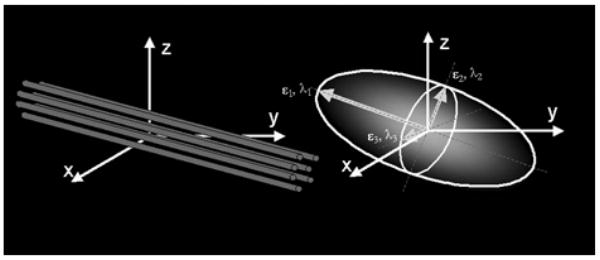
\includegraphics[width=9cm,height=5cm]{images/nihms26625f2.jpg}\hfill
%% \else
      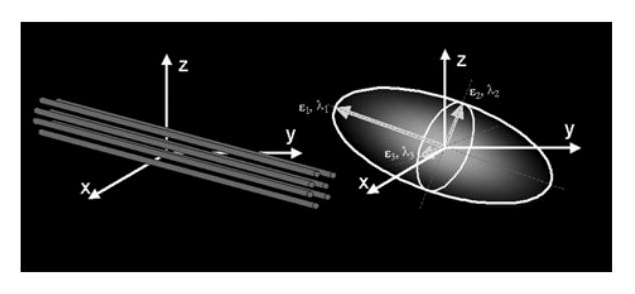
\includegraphics[width=9cm,height=5cm]{images/nihms26625f2.eps}\hfill

%% \fi
   \end{center}
   \caption{\label{nihms26625f2} Diffusion displacement distributions for the diffusion tensor. The diffusion is highly anisotropic in fibrous tissues such as white matter and the direction of greatest diffusivity is generally assumed to be parallel to the local direction of white matter~\cite{citeulike:1695483}.}
\end{figure}

The display, meaningful measurement, and interpretation of 3D image data with a $3 \times 3$ diffusion matrix at each voxel is a challenging or impossible task without simplification of the data. Consequently, it is desirable to distill the image information into simpler scalar maps. The two most common measures are the trace and anisotropy of the diffusion tensor. The trace of the tensor, or sum of the diagonal elements of $\Bar{\bar{D}}$, is a measure of the magnitude of diffusion and is rotationally invariant. The MD (often called the apparent diffusion coefficient or ADC) is used in many published studies and is simply the trace divided by three (MD = Tr/3), which is equivalent to the average of the eigenvalues. Many measures of anisotropy have been described, most of which are rotationally invariant.}

\paragraph{Diffusion tensor imaging: Concepts and applications~\cite{lebihan2001}}{
Water molecules move in the brain on average over distances around 10~$\mu$m, bouncing, crossing, or interacting with many tissue components such as cell membranes, fibers, or macromolecules.

The overall effect observed in a diffusion MRI image voxel of several mm$^{3}$ reflects, on a statistical basis, the displacement distribution of the water molecules present within this voxel. The observation of this displacement distribution may thus provide unique clues to the structure and geometric organization of tissues.

This anisotropy may result from a peculiar physical arrangement of the medium (such as in liquid crystals) or the presence of obstacles that limit molecular movement in some directions. As diffusion is encoded in the MRI signal by using magnetic field gradient pulses (8), only molecular displacements that occur along the direction of the gradient are visible. The effect of diffusion anisotropy can then easily be detected by observing variations in the diffusion measurements when the direction of the gradient pulses is changed. This is a unique, powerful feature not found with usual MRI parameters, such as T1 or T2.

Diffusion anisotropy in white matter originates from its specific organization in bundles of more or less myelinated axonal fibers running in parallel, although the exact mechanism is still not completely understood: diffusion in the direction of the fibers is faster than in the perpendicular direction. It quickly appeared that this feature could be exploited to map out the orientation in space of the white matter tracks in the brain using a color scale, assuming that the direction of the fastest diffusion would indicate the overall orientation of the fibers.

To determine the diffusion tensor fully, one must first collect diffusion-weighted images along several gradient directions, using diffusion-sensitized MRI pulse sequences such as echoplanar imaging (EPI). As the diffusion tensor is symmetric, measurements along only six directions are mandatory (instead of nine).}

\section{Conductivity tensor}

\paragraph{Conductivity tensor mapping of the human brain using diffusion tensor MRI~\cite{Tuch25092001}}{
Here, using an effective medium approach, we show how the electrical conductivity tensor of tissue can be quantitatively inferred from the water self-diffusion tensor as measured by diffusion tensor magnetic resonance imaging.

Excitable tissues such as nerve and muscle mediate communication through electrical currents. These endogenous currents are capable of generating electromagnetic fields sufficiently large to be measured outside of the body by using, for example, electro/magnetoencephalography (EEG/MEG) in the case of the brain or electro/magnetocardiography (ECG/MCG) for the heart.

Efforts to develop an imaging modality to quantitatively measure the electrical conductivity of tissue noninvasively have largely been thwarted by anatomical and biophysical barriers: the organ of interest can be shielded by highly resistive barriers such as the bony tissue of the skull, and the tissue can exhibit significant reactance, anisotropy, and microstructural heterogeneity.

DTI employs an pulsed-gradient spin echo to measure the self-diffusion tensor of water in the tissue (13). The hypothesized relationship between electrical conductivity and water self-diffusion in tissue is prompted by the observation that, although there is no fundamental relationship between the two transport modes in free solution, in a structured medium such as tissue the two processes are related through mutual respect for the boundary conditions imposed by the tissue geometry.

 To derive the cross-property relation between the conductivity and diffusion tensors in brain tissue, the approach we adopt here is to estimate the statistical moments of the microstructure from the observed diffusion tensor, and then derive the conductivity tensor from the estimated moments. We assume in the following that the cell membrane is freely permeable to water and impermeable to charge-carriers on the experimental time scale ($\sim$~50~ms). Following Sen and Torquato.
 
The two-phase model consisting of an inclusion phase embedded in a host phase is particularly amenable to describing biological tissues because the extracellular space can be taken as the host phase and the intracellular space as the inclusion phase.
 
Following Sen and Torquato (22), the effective transport tensor $\Bar{\bar{\Lambda}}$, denoting either the effective electrical conductivity tensor $\Bar{\bar{\sigma}}$ or the diffusion tensor $\Bar{\bar{D}}$, for a two-phase anisotropic medium of arbitrary topology is given by
%% 
%% eq1
%% 
where $\varphi_{i}$ is the inclusion (intracellular) volume fraction, $\Bar{\bar{U}}$ is the identity tensor, and $\lambda_{i}$ and $\lambda_{e}$ are, respectively, the inclusion (intracellular) and host medium (extracellular) transport coefficients; for example, in the case of diffusion $d_{i}$ is the intracellular diffusion coefficient and $d_{e}$ is the extracellular diffusion coefficient. Similarly, $\sigma_{i}$ is the intracellular conductivity value and $\sigma_{e}$ is the extracellular conductivity. The dimensionless contrast factors $\beta$ and $\Bar{\bar{B}}$ are defined as

%% 
%% eq2 et eq3
%% 

The rank-2 tensors $A_{n}^{(i)}$ contain the microstructure information and are defined as integrals over the $n$-point probability functions $S_{n}^{i}$, which give the probability of finding $n$ points within the inclusion (intracellular) phase. Exact expressions for $A_{n}^{(i)}$ are available in ref. 22.
By setting $A_{1}^{(i)} = - \phi_{i} \Bar{\bar{U}}$, the first term on the right-hand side of Eq. 1 can be embedded in the sum to give 

%%
%% eq 4
%% 

where we have defined $\beta_{\lambda} = \beta(\lambda_{i}, \lambda_{e})$ \dots

{\bf Results} \\
The full fractional linear relationship (Eq. 11) was fit to the conductivity and diffusion data, as was a linear relationship of the form $\sigma_{nu} = k(d_{\nu} - d_{\varepsilon})$ for comparison. The linear fit yielded $k = 0.844 \pm 0.0545$~S.s/mm$^{3}$ and $d_{\varepsilon} = 0.124 \pm 0.0540~\mu$m$^{2}$/ms $r^{2} = 0.945$.
}

%
\chapter{Numerical method for modelling of physical processes}
\minitoc
bla

\newpage

%-------------------------------------------------------------------------------

\section{Finite element methode\label{FEM}}

The \FEM{} is a method of approximating the solution of \PED{} which is constructed from an equivalent formulation of the problem. This equivalent formulation is called {\it weak formulation}\index{weak formulation}. The general approach of the \FEM{} can be summarized in the following way: 

\begin{itemize}
\item We have a \PED{} with boundary conditions. We multiply this equation by a test function, we integrate over the entire simulation domain.
\item The second step is to make a partial integration in order to obtain the weak formulation.
\item At this stage, the domain discretization is essential (triangular or quadrilateral in two dimensions, tetrahedral and hexahedral in three dimensions). 
\end{itemize}


\newpage

%-------------------------------------------------------------------------------

\section{Mathematical background}

The method principal is to approach on a domain $\Omega$, the solution of a \PED{} with boundary conditions on the edges of $\partial\Omega$ with local fields. Local fields defined on each subdomain $\Omega_{i}$ are generally polynomial interpolation. The overall solution is the concatenation of all local fields. The quality of the solution depends on the division of the sub-domain.

\subsection{Weak formulation}

\subsection{Galerkin method}

\subsection{Introduction to FEM}

\newpage

%-------------------------------------------------------------------------------

\section{Sparse matrices}

\subsection{Sparse matrix formats}
\subsubsection{Coordinate list (COO)}
\subsubsection{Compressed sparse row (CSR or CRS)}

\newpage

%-------------------------------------------------------------------------------

\section{Krylov space}

Goal $Ax = b$\\
Say something we don't care about direct methods. We only work on iterative methods (Krylov space)\\

Development: \\
$LU$ factorisation\\


A Krylov method, named after Aleksey Nikolaevich Krylov (1863 - 1945) was a Russian naval engineer, applied mathematician, is a method that solves the system $Ax = b$ by repeatedly performing matrix-vector multiplications involving $A$. this excludes methods like biconjugate gradient method that also require matrix-vector multiplications involving the conjugate transpose $A^{*}$.\\
We will show that the solution to a nonsingular linear system $Ax = b$ lies in a Krylov space whose dimension is the degree of the minimal polynomial of $A$\footnote{The minimal polynomial of a matrix $A$ is defined by: $P(A) = \alpha_{0}I + \alpha_{1}A + \cdots \alpha_{k}A^{k} = 0$ }. 

\paragraph{Theorem}{\it If the minimal polynomial of the nonsingular matrix $A$ has degree $k$, then the solution to $Ax = b$ lies in the space $\mathcal{K}_{k}(A, b)$.}

Along the caracteristic polynomial, the minimal polynomial provide the eigenvalues spectrum. Then, the smallest Krylov space containing $x$ is $k$, the degree of the minimal polynomial of $A$. If the minimal polynomial has low degree then the Krylov space containing the solution is small, and a Krylov method converge fast. Eigenvalues play a central role to ensuring existence and uniqueness of Krylov solutions. \\

\paragraph{Definition:}{\it Given a nonsingular matrix $A \in \mathbb{C}^{m,m}$ and $y \ne 0 \in \mathbb{C}^{m}$ , the nth Krylov subspace $\mathcal{K}_{n}(A,y)$ generated by $A$ and $y$ is

$$
\mathcal{K}_{n}(A,y) = span\{y, Ay, \cdots , A^{n-1}y\}
$$
}

\subsection{Arnoldi iteration}

The problem of solving the system $Ax = b$ is closely related to sparse matrices eigenvalues research problem. We will briefly develop the eigenvalues problem (Arnoldi iteration), and then adapt it to our system $Ax = b$ problem. Arnoldi method finds the eigenvalues of general (possibly non-Hermitian) matrices; an analogous method for Hermitian matrices is the Lanczos iteration. The Arnoldi iteration was invented by W. E. Arnoldi in 1951.\\
The Arnoldi's method is based on the {\it power iteration algorithm} (iteration Von Mises), we will describe later. Indeed, the construction successive powers of a matrix A will give us the eigenvector $| \lambda_{1} >$ of the dominant eigenvalue $\lambda_{1}$. At first we will describe the Gram-Schmidt algorithm, which is the base line for all the following algorithm.

\paragraph{Gram-Schmidt algorithm}{ The Gram-Schmidt method allows, starting from a set of random vectors $\{v_{1}, v_{2}, \dots, v_{n}\}$, to construct an orthogonal basis $\{u_{1}, u_{2}, \dots, u_{n}\}$ or $e_{1}, e_{2}, \dots, e_{n}$ orthonormal.

$$
\begin{array}{rclcl}
u_{1} & = & v_{1} & \Leftrightarrow& e_{1} = u_{1} / \| u_{1} \| \\
u_{2} & = & v_{2} - P_{u_{1}}(v_{2})& \Leftrightarrow& e_{2} = u_{2} / \| u_{2} \| \\
u_{3} & = & v_{2} - P_{u_{1}}(v_{3}) - P_{u_{2}}(v_{3})& \Leftrightarrow& e_{3} = u_{3} / \| u_{3} \| \\
\vdots &&&& \\
u_{n} & = & v_{n} - \sum_{i = 1}^{n-1} P_{u_{i}}(v_{n})& \Leftrightarrow& e_{n} = u_{n} / \| u_{n} \| \\
\end{array}
$$

The idea is to orthogonalize the vector $v_{n}$ by removing its projections componant on the basis $e_{1}, e_{2}, \dots, e_{n-1}$.
}

\paragraph{Power iteration algorithm}{

L'algorithme de power iteration suit le même principe que l'algorithme Gram-Schmidt. L'algorithme commence avec un vecteur $| b_{0} >$ avec des composantes aléatoires. Le vecteur suivant est construit de la façon suitante:

$$
| b_{k+1} > = \frac{A | b_{k} >}{\|| b_{k} >\|}
$$

Nous atteignons la convergence quand $| b_{k} > = | b_{k+1} > / \| | b_{k+1} > \|$. En d'autres termes, si nous normailsons à chaque étape, nous avons:

$$
| e_{k} > = \frac{| b_{k} > }{ \| | b_{k} > \|}
$$

Alors:

$$
| b_{k+1} > = A | e_{k} > and | e_{k+1} > = \frac{| b_{k+1} > }{ \| | b_{k+1} > \|}
$$

Nous atteignons la convergence quand $| e_{k+1} > = | e_{k} > = | \lambda_{1} >$.  Ce qui veut dire:

$$
\underset{\lambda_{1}}{\| | b_{k+1} > \|}| e_{k+1} > = A| e_{k} > \Leftrightarrow \lambda_{1} | \lambda_{1} > = A| \lambda_{1} >
$$
}

L'algorithme de {\it Power iteration} est généralisé pour créer l'espace de Krylov.

%http://en.wikipedia.org/wiki/Arnoldi_iteration

$$
H_{n} = \left(
\begin{array}{ccccc}
h_{1,1} & h_{1,2} & h_{1,3} & \cdots & h_{1,n} \\
h_{2,1} & h_{2,2} & h_{2,3} & \cdots & h_{2,n} \\
0       & h_{3,2} & h_{3,3} & \cdots & h_{3,n} \\
\vdots  & \ddots  & \ddots  & \ddots & \vdots  \\
0       & \hdots  & 0       & h_{n,n-1} & h_{n,n} \\
\end{array}
\right)
$$

$$
\tilde{H}_{n} = \left(
\begin{array}{ccccc}
h_{1,1} & h_{1,2} & h_{1,3} & \cdots & h_{1,n} \\
h_{2,1} & h_{2,2} & h_{2,3} & \cdots & h_{2,n} \\
0       & h_{3,2} & h_{3,3} & \cdots & h_{3,n} \\
\vdots  & \ddots  & \ddots  & \ddots & \vdots  \\
0       & \hdots  & 0       & h_{n,n-1} & h_{n,n} \\
0       & \hdots  & \hdots  & 0         & h_{n+1,n} \\
\end{array}
\right)
$$

\subsection{GMRES}


\subsection{Preconditioners}



\newpage

%-------------------------------------------------------------------------------

\section{FEniCS}

\newpage

%-------------------------------------------------------------------------------

\section{To review}











Dans les applications de calcul, du type éléments finis, plus le maillage est dense plus la précision du calcul augmente. Cependant, la quantité de temps nécessaire à l'accomplissement d'un calcul basé sur un maillage est souvent proportionnelle au nombre d'éléments du maillage. Un compromis doit donc être trouvé entre la précision et le temps de calcul. 



La méthode des éléments finis permet la résolution approchée de systèmes d'équations aux dérivées partielles, en cherchant une solution approchée du problème qui s'exprime comme combinaison linéaire d'un ensemble de fonctions élémentaires. Le choix de l'ensemble des fonctions élémentaires est très important pour la convergence de cette méthode, et est en général guidé par un maillage du domaine dans lequel on cherche à résoudre le système d'équations. A chaque élément du maillage est associé un petit ensemble de fonctions élémentaires adapté au problème, et la solution approchée est exprimée comme combinaison linéaire des fonctions élémentaires de tous les éléments du maillage. Pour calculer la solution approchée, il suffit alors d'inverser un système d'équations algébriques linéaires.

%
%
%
%
%\part{Int�raction dans la mati�re}
%\chapter{\'Equation du transport}
%\minitoc
%%\include{chapters/InteractionParticules}
%%
%
%
%
%\part{Appendix}
%\appendix
%\chapter{Formules et Fonctions de Green}
%\minitoc
%%\include{appendix/FonctionsGreen}
%
%
%
\backmatter
%
%
%
\chapter{Conclusion}
%\include{chapters/Conclusion}
%
%
%
\newpage
%
%
%
\bibliographystyle{unsrt}
\bibliography{Fijee} 
%
%
%
\printindex
%
%
%
\newpage
\clearpage
\end{quote}
\end{document}
